\chapter{Introdu\c{c}\~{a}o} \label{chapter:intro}
Nas últimas décadas os jogos eletrônicos estiveram presentes no cotidiano das pessoas e acompanharam o crescimento e amadurecimento de seus usuários, evoluindo para plataformas cada vez mais poderosas como PS3 e Xbox 360~\cite{moore2011basics}. A~\textit{Entertainment Software Association}, que é uma associação formada pelas principais fabricantes americanas de jogos eletrônicos, publicou uma pesquisa constatando que no ano de 2011 os jogadores americanos possuíam em média 37 anos e 29$\%$ tinham mais de 50 anos.

Os jogos para a prática de exercício físico doravante \textit{Exergames} se tornaram extremamente populares e estudos já comprovam seus benefícios em relação ao aumento da atividade física ~\cite{baran08}. A principal motivação para o seu desenvolvimento se deve ao estilo de vida atual das pessoas, que fazem uso de diversos dispositivos eletrônicos em seu cotidiano diminuindo a atividade física, ocasionando numa redução da qualidade de vida dos indivíduos~\cite{maitland}. Por esse motivo, pretende-se com o uso destes jogos motivar a prática da atividade física através de execução de movimentos específicos que permitem a queima de calorias e consequentemente uma melhora da saúde~\cite{Suhonen:2008:SFE:1457199.1457204}. A prática da educação física num ambiente controlado como um jogo eletrônico é segura pois permite que as pessoas realizem movimentos específicos. Dependendo do ambiente do jogo é possível inclusive auxiliar na correção postural motivacional para a prática do exercício físico, fornecendo uma avaliação da atividade física desempenhada~\cite{Hardy2011,vaghetti2011,Suhonen:2008:SFE:1457199.1457204}.  %Contudo, estudos indicam que os jogos para exercício físico não conseguem o uso contínuo de seus usuários. Normalmente os jogadores tendem a usá-los durante 4 semanas e por conta dos movimentos repetitivos ficam desmotivados a jogarem mais vezes ~\cite{sinclair07}.

Desde 2005 os jogos eletrônicos fazem uso de dispositivos como acelerômetros, giroscópio, dispositivos de captura de movimento possibilitando que o usuário fique mais imerso no universo do jogo através da análise de seus movimentos. Como o uso desses dispositivos se encontra embutido no contexto do jogo, possivelmente o usuário não sentiria desconforto caso os jogos eletrônicos fossem utilizados para monitorar seus dados motores. Desta forma, a abordagem \textit{GAHME} pretende realizar o monitoramento motor por meio de um jogo eletrônico que captura, processa dados e identifica sintomas de distúrbios do movimento.

A presente pesquisa parte do pressuposto que os sintomas motores podem ser quantificados por sensores de movimento~\cite{visionbased2009,patel_monitoring_2009,bachlin_parkinsons_2009} e que estes podem ser usados dentro de um cenário de jogo eletrônico. Este trabalho agrega a capacidade de monitorar sintomas motores do usuário dentro de um ambiente de jogo eletrônico e, por meio destes, os usuários podem integrá-lo na rotina aumentando assim a frequência do monitoramento dos dados motores.


\section{Problemática}\label{section:problematica}
%Para a identificação do problema foi realizado inicialmente uma Revisão Bibliográfica sobre os temas IEEE ~\cite{ieee}, ACM ~\cite{acm}, PubMed ~\cite{pubmed}, Scielo ~\cite{scielo} além de Congressos Brasileiros em Informática na Saúde ~\cite{cbis} e do Workshop de Informática Médica evento promovido pela ~\cite{sbc}.
%
%A Revisão da Literatura teve como objetivo buscar trabalhos na área de Computação Aplicada a Saúde que tivessem o objetivo de realizar monitoramento de dados de saúde além de um estudo complementar nas diretrizes médicas que iriam proporcionar o suporte científico nesta área. Essa etapa teve como objetivo inicial identificar problemas nesses trabalhos que pudessem ser solucionados através da presente proposta.

Os sistemas de monitoramento motor fazem uso de sensores sem fio e vestíveis (\textit{wearable}) que podem ser incorporados na roupa ou no corpo do usuário. Esses sistemas permitem um monitoramento contínuo dos dados motores. Porém, os dispositivos são considerados invasivos e estereotipados~\cite{aarh10}, pelos usuários o que inibe sua disseminação e uso~\cite{alemdar}. Como pode ser visto nos trabalhos que se propõem a monitorar dados motores~\cite{LeMoyne2009,patel_monitoring_2009} (Figuras: \ref{fig:quantif-parkinson},\ref{fig:patel-shimmer}), percebe-se a dificuldade de integrar esses dispositivos à rotina dos usuários, e impacta diretamente na possibilidade de realizar um monitoramento frequente dos sintomas motores.

\begin{figure}
 \centering
 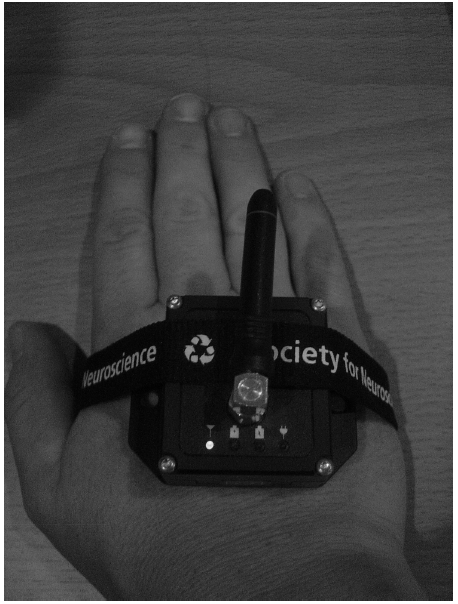
\includegraphics[scale=0.3]{./img/quantif-parkinson.png}
 % matrixargseg.png: 296x162 pixel, 100dpi, 7.52x4.11 cm, bb=0 0 213 117
 %\caption{Estágio desenvolvimento de jogos ~\cite{fullerton2008game}}
\caption[\textit{G-Link Wireless Accelerometer} - Instrumento usado no trabalho de LeMoyne para quantificar o tremor da Doença de Parkinson]{\textit{G-Link Wireless Accelerometer} - Instrumento usado no trabalho de LeMoyne~\cite{LeMoyne2009} para quantificar o tremor da Doença de Parkinson} 
%  \caption{Estágio desenvolvimento de jogos}
 \label{fig:quantif-parkinson}
\end{figure}

\begin{figure}
 \centering
 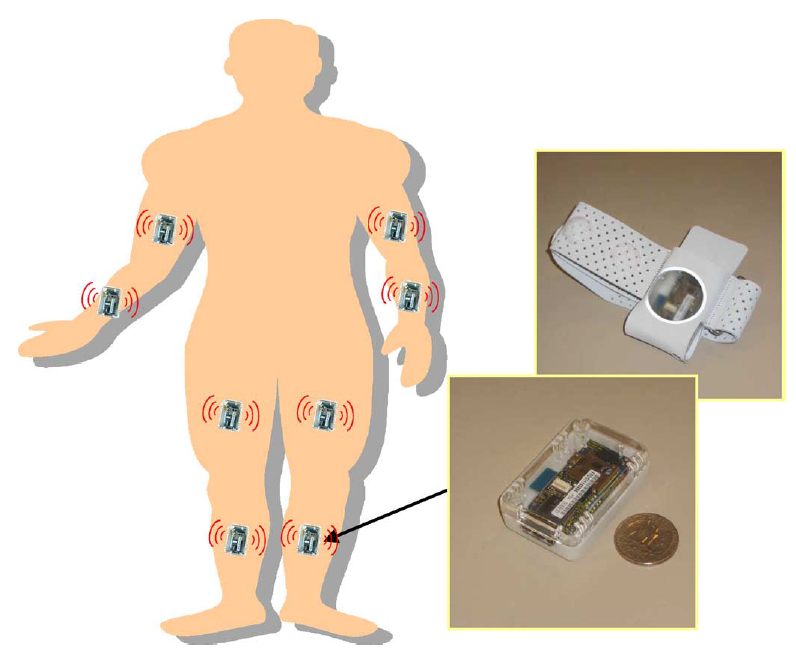
\includegraphics[scale=0.3]{./img/patel-shimmer.png}
 % matrixargseg.png: 296x162 pixel, 100dpi, 7.52x4.11 cm, bb=0 0 213 117
 %\caption{Estágio desenvolvimento de jogos ~\cite{fullerton2008game}}
\caption[Disposição dos Sensores de Movimento (SHIMMER) no corpo no trabalho de Patel]{\textit{Disposição dos Sensores de Movimento (SHIMMER) no corpo no trabalho de Patel ~\cite{patel_monitoring_2009}}}
%  \caption{Estágio desenvolvimento de jogos}
 \label{fig:patel-shimmer}
\end{figure}

Em um trabalho mais recente, LeMoyne ~\cite{lemoyne2010} conseguiu quantificar os sintomas dos tremores da Doença de Parkinson (\ac{dp}) usando um Apple iPhone (Figura \ref{fig:iphone-tremor}). Como os \textit{smartphones} já estão integrados à rotina diária do usuário, poderia ser uma solução para esse contexto. Contudo, essa solução necessita que o usuário abra o aplicativo no telefone e ponha o dispositivo no torso da mão em diferentes momentos do dia. Percebe-se então que, nesse contexto, o usuário modifica sua rotina diária para prover os dados relativos à saúde.

\begin{figure}
 \centering
 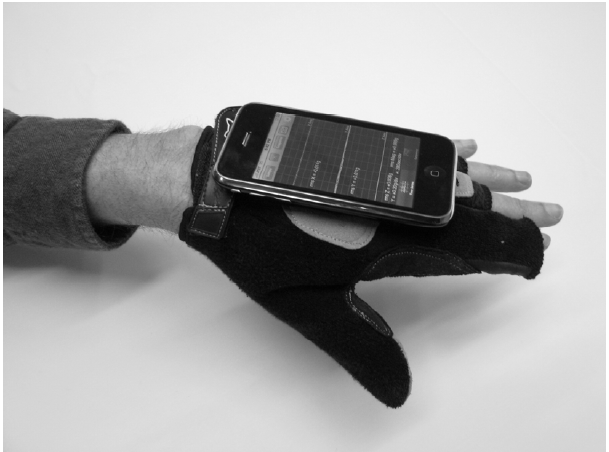
\includegraphics[scale=0.3]{./img/moyne-iphone.png}
 % matrixargseg.png: 296x162 pixel, 100dpi, 7.52x4.11 cm, bb=0 0 213 117
 %\caption{Estágio desenvolvimento de jogos ~\cite{fullerton2008game}}
\caption[Aplicação para iPhone que caracteriza sinais de tremor]{Aplicação para iPhone que caracteriza sinais de tremor ~\cite{lemoyne2010}}
%  \caption{Estágio desenvolvimento de jogos}
 \label{fig:iphone-tremor}
\end{figure}


%em diferentes momentos do dia dentro de um ambiente de jogo eletrônico o qual pode estar integrado em sua rotina diária.
Partindo da necessidade de monitorar dados motores de uma forma não invasiva por intermédio de sensores de movimento, pretende-se neste trabalho usar jogos eletrônicos como forma de \textbf{motivar} e abstrair o monitoramento de dados de saúde, pondo o usuário longe do \textbf{contexto de tratamento da saúde}. Esse estudo analisa possíveis mecanismos de monitoramento da saúde motora durante um período lúdico e descontraído como um jogo eletrônico.

A Figura \ref{fig:problematica} sumariza os passos usados para a identificação do \textbf{problema} e a \textbf{Proposta da Tese} que elabora alternativas a esse problema.

\begin{figure}[!H]
 \centering
 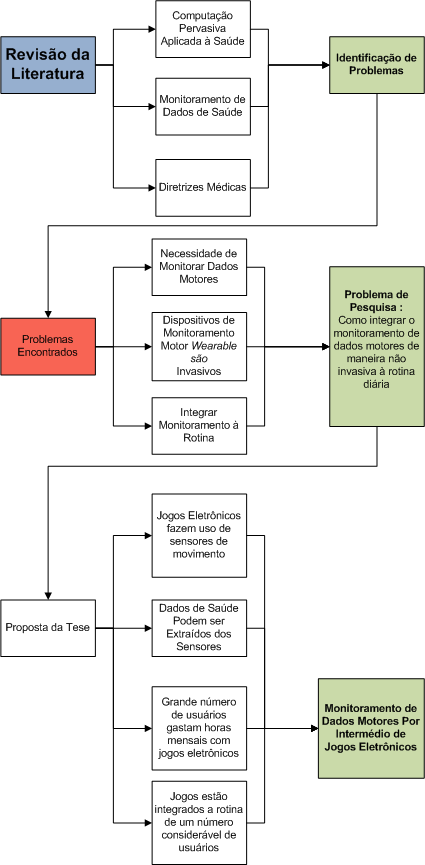
\includegraphics[scale=0.8]{./img/problematica.png}
 % matrixargseg.png: 296x162 pixel, 100dpi, 7.52x4.11 cm, bb=0 0 213 117
 %\caption{Estágio desenvolvimento de jogos ~\cite{fullerton2008game}}
\caption{Processo de Identificação do Problema e Proposta da Tese}
%  \caption{Estágio desenvolvimento de jogos}
 \label{fig:problematica}
\end{figure}
\FloatBarrier

\section{Objetivos}
\subsection{Objetivo Principal}
Neste trabalho, tem-se como objetivo a concepção de uma abordagem computacional para o monitoramento de dados motores. Pretende-se usar jogos eletrônicos como forma de \textbf{motivar} e abstrair o monitoramento de dados de saúde de uma maneira \textbf{não invasiva} e longe do \textbf{contexto de tratamento de saúde}.


%Partindo da necessidade de monitorar dados motores de uma forma não invasiva por intermédio de sensores de movimento, pretendemos usar jogos eletrônicos como forma de \textbf{motivar} e abstrair o monitoramento de dados de saúde de forma \textbf{não invasiva} e longe do \textbf{contexto de tratamento de saúde}.
Nesta pesquisa, pretende-se identificar mecanismos que permitam monitorar a saúde durante um período divertido e descontraído, usando jogos eletrônicos que capturem, armazenem  e processem esses dados. Essa pesquisa tem como objetivo demonstrar a alternativa de realizar o monitoramento de dados de saúde por intermédio de jogos eletrônicos.
%Em um primeiro momento, serão verificados junto a profissionais de saúde a relevância desse trabalho e se este poderia auxiliar no monitoramento dos sintomas parkinsonianos.

Para atingir estes objetivos, foram elencadas e testadas as seguintes hipóteses:
	\begin{description}
	\item[H1] O acompanhamento de sintomas motores, integrados à rotina diária do paciente traz benefícios ao tratamento e qualidade de vida do mesmo do ponto de vista do profissional da saúde.
	\item[H2] É possível capturar dados motores por meio de sensores de movimento utilizados em jogos eletrônicos. Esses dados auxiliam no acompanhamento de doenças com comprometimento motor.
	\item[H3] É possível desenvolver um jogo que tenha mecanismos de captura de dados motores embutidos, e que permita monitorar e quantificar esses dados de maneira não-invasiva.
	\end{description}
	
\subsection{Objetivos Específicos}
\begin{enumerate}
		\item Identificar a importância de realizar monitoramento de dados de saúde em diferentes momentos do dia junto a uma comunidade de profissionais de saúde.
		\item Usar algoritmos de classificação em base de dados de saúde já consolidadas, para desenvolver e testar novas abordagens de monitoramento, além de aumentar o número de casos pesquisados.
		\item Identificar viabilidade técnica para mensurar dados de saúde por meio de sensores de movimento utilizados em jogos eletrônicos.
		\item Definir e implementar a arquitetura de software de uma abordagem que consiga: adquirir, processar, classificar e transformar em informações de saúde motora os sinais biomecânicos de usuários obtidos a partir de um arcabouço de desenvolvimento de jogos eletrônicos.
		%\item Definir processo de desenvolvimento de jogos que consiga realizar o monitoramento de dados de saúde não-invasiva ao usuário;
		\item Realizar experimentos no sentido de validar as hipóteses descritas anteriormente.
\end{enumerate}

\section{Metodologia}
A metodologia de pesquisa deste trabalho possui aspectos qualitativos que permitem identificar a importância da pesquisa junto à comunidade de especialistas da área de saúde. Além disso, usam-se aspectos quantitativos que demonstram que a abordagem definida consegue diferenciar indivíduos diagnosticados com a ~\ac{dp}, perante indivíduos sem o diagnóstico estabelecido por meio de dados capturados por sensores de movimento usados em jogos. Ao final, é avaliado o resultado de um questionário ~\ac{gqm} junto a possíveis usuários. Logo, o desfecho da pesquisa se fez com resultados qualitativos e quantitativos.

\begin{enumerate}

\item{Realizar revisão bibliográfica e coleta de requisitos junto a profissionais de saúde.}

\item{Definir a abordagem \textit{GAHME - Health Monitor Environment}, baseada em captura de dados motores através de sensores de movimento utilizando jogos eletrônicos e processamento dos dados para transformar dados motores em informações.}

\item{Validar o uso de sensores para classificação dos dados através:} 
	\begin{itemize}
		\item Base de dados contendo a~\ac{fvrs} capturada por sensores de movimento que contém duas classes de dados indivíduos diagnosticados com a \ac{dp} e o grupo de controle. Esses dados foram classificados utilizando-se da Análise dos Componentes Principais (PCA).
		\item Estudo analítico de caso-controle com indivíduos diagnosticados com a doença de parkinson, e sem o diagnóstico estabelecido capturados por sensores de movimento de usados em jogos eletrônicos. Esses dados foram classificados utilizando de~\ac{svm} com Kernel Linear.
		\item O resultado dessa pesquisa demonstra que é possível adquirir dados motores utilizando esta abordagem e consequentemente valida a hipótese \textit{H2}.
	\end{itemize}
\item{Definir a arquitetura de software que viabiliza tecnicamente a abordagem \textit{GAHME} onde foi possível definir um arcabouço de software que encapsula o desenvolvimento de jogos com essa abordagem.}

\item{Validar a solução \textit{GAHME} do ponto de vista computacional. A solução foi validada através da implementação da arquitetura e desenvolvimento de jogos com base na arquitetura. Com jogos, demonstrou-se ser possível realizar monitoramento de dados motores de forma não invasiva, ou seja, sem os jogadores perceberem que estão fornecendo dados de saúde.}

\item{A importância da entrevista semi-estruturada junto a profissionais de saúde é alinhar a teoria junto à prática do acompanhamento de pacientes com \textit{déficit} motor.  Os profissionais foram indagados sobre a melhora na tomada de decisão quanto ao acompanhamento dos sintomas, caso fosse possível visualizar parâmetros motores como velocidade angular, amplitude do movimento dos braços e dessa maneira acompanhar a evolução dos pacientes. Procurou-se encontrar, do ponto de vista do profissional de saúde, a importância do monitoramento de dados de saúde e os benefícios trazidos por este através de uma abordagem de pesquisa qualitativa. Com esta pesquisa foi possível validar a hipótese \textit{H1} que consiste de verificar a importância do acompanhamento de sintomas motores integrados à rotina diária do paciente.}
    
\item{Definir um conjunto de atividades que permitam o desenvolvimento de jogos voltados para o monitoramento de dados de saúde (\textit{GAHME}). Desta maneira, pretende-se com esse trabalho disseminar o conhecimento adquirido a partir de um conjunto de passos que tornem exequível o desenvolvimento de um \textit{GAHME}.}

\end{enumerate}

%\subsection{Desenho da Pesquisa} \label{sec:desenho_pesquisa}
%Para uma melhor compreensão da pesquisa temos o Desenho da Pesquisa a ser realizada na Figura \ref{figure:desenho_pesquisa} e a descrição de cada um dos passos.
%
%A Problemática desse trabalho, já foi descrita na Seção \ref{section:problematica}. A revisão da literatura consistiu de uma descrição sobre a doença estudada como estudo de caso (Doença de Parkinson) que está descrito no Capítulo \ref{section:doenca_parkinson}, bem como da possibilidade de integrar o monitoramento da doença de Parkinson por intermédio de jogos eletrônicos.
%
%\begin{figure}[!htp]
    %\centering
    %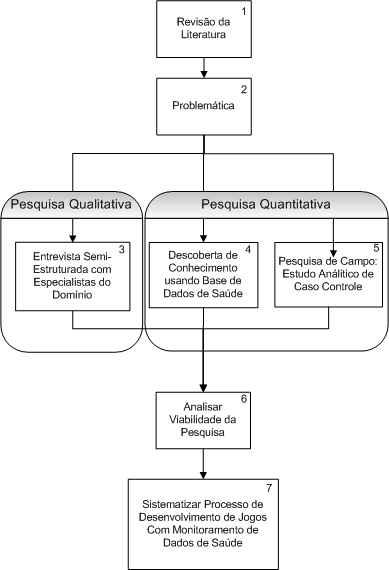
\includegraphics[width=.7\textwidth]{./img/metodologia-pesquisa.png}
    %\caption{Desenho da Pesquisa}
    %\label{figure:desenho_pesquisa}
%\end{figure}

%\subsection{Pesquisa Qualitativa}
%Essa pesquisa tem como objetivo identificar a importância de realizar o monitoramento de dados de saúde por intermédio jogos eletrônicos. Em um primeiro momento, serão verificados junto a comunidade médica a relevância desse trabalho e se este poderia auxiliar no monitoramento dos sintomas parkinsonianos.
%
%Os pesquisadores que adotam a abordagem da pesquisa qualitativa a fazem por sua flexibilidade, sem regras rígidas, aplicáveis a uma ampla gama de casos e formalizações pré-definidas, possibilitando a construção de modelos abrangentes \cite{Gom00}.
%Nesse estudo a pesquisa qualitativa está orientada a um estudo de caso, partindo da análise das expressões e comportamento das pessoas. Na busca por entender os fenômenos sociais complexos, o estudo de caso permite uma investigação significativa nas mudanças desses processos\cite{Yin05}.
%
%\subsubsection{Entrevista Semi-Estruturada Com Especialistas do Domínio (3)}\label{section:entrevista_semi-estruturada}
%
%O objetivo deste procedimento foi entender como é feito o acompanhamento dos sintomas da doença de parkinson juntamente aos profissionais de saúde (neurologistas que prescrevem a dosagem medicamentosa e fisioterapeutas que fazem o acompanhamento motor do paciente ao longo de seu tratamento). Os mesmos foram indagados se poderia haver melhora na tomada de decisão caso eles pudessem acompanhar o surgimento dos sintomas em diferentes momentos do dia por intermédio de um monitoramento frequente dos sintomas. Procurou-se encontrar dentro do contexto de estudo, a importância do monitoramento de dados de saúde e os benefícios trazidos por este.
%
%As entrevistas foram realizadas de maneira presencial, onde primeiramente fez-se perguntas não estruturadas e havendo uma maior estruturação no decorrer da entrevista com a preocupação de que seja evitada a referência do entrevistador seja sobre os pontos de vista do entrevistado conforme prega o método científico \cite{FLI04}. Durante a pesquisa foi utilizado recursos de gravação, de modo a facilitar a transcrição dos dados coletados.
%
%\subsection{Descoberta de Conhecimento usando Base de Dados de Saúde}
%Para esse estudo, foram utilizados dados do \textit{PhysioBank} ~\cite{physionet}. O \textit{PhysioBank} armazena sinais fisiológicos e dados relacionados a comunidade de pesquisa biomédica, incluindo sinais vitais, motores de indivíduos saudáveis e de pacientes com uma variedade de sintomas como distúrbios neurológicos ou envelhecimento.
%
%A análise dos dados da \textit{Parkinson Disease Database} ~\cite{physionet}, incluiu 50 pacientes de Parkinson e 50 indivíduos que não possuíam desenvolvido a doença (segundo as informações fornecidas pela própria base de dados). Foram calculados, normalizados e escalonados em 80 \textit{frames} um total de 120 ciclos de marcha (Seção \ref{section:analise_marcha}) que foram usados para efetuar a técnica de aplicar a técnica \textit{eigengaits} ~\cite{medeiros2013} que é uma adaptação da Análise dos Componentes Principais que será explicada na Seção \ref{section:analise_marcha_pca}.
%
%\subsection{Estudo Analítico Caso Controle com \textit{Support Vector Machine} (SVM)}
%Esta etapa da pesquisa foi pautada pelo protocolo de pesquisa submetido à avaliação do Comitê de Ética da UFCG, somente após a aprovação deste (\textbf{CAAE: 14408213.9.1001.5182}) é que os dados foram coletados.
%Os resultados que se desejou alcançar com a pesquisa foi o descobrimento de mecanismos para a identificação e classificação de duas classes de indivíduos os  diagnosticados com a doença de parkinson ante indivíduos sem o diagnóstico estabelecido. Durante a pesquisa também analisou-se o sensor de movimento MS-Kinnect ~\cite{kinnect2013} para avaliar a possibilidades de aquisição de dados de saúde baseada na Cinemática Linear do Movimento Humano.
%
%O propósito dessa classificação é explorar a possibilidade de obter dados de saúde de forma contínua e não invasiva a partir de um sensor de captura de movimento usado em jogos eletrônicos (Ms-Kinnect).
%Os dados adquiridos foram processados extraindo características do movimento angular e postos em uma máquina de de Aprendizagem do tipo \textit{Suppport Vector Machine} para realizar a classificação das duas classes de dados.

\section{Trabalhos Relacionados}\label{section:jogos_saude}
O estilo de vida atual possui diversos dispositivos eletrônicos e formas de entretenimento que não privilegiam a atividade física por esse motivo houve uma diminuição de indivíduos que praticam exercícios físicos e consequentemente tenham uma vida mais saudável~\cite{maitland}. Com o objetivo de usar a tecnologia para motivar a execução de exercícios físicos, pesquisadores da área de jogos para saúde buscam apoiar a essa prática com o uso de jogos para exercício físico, como também tentam mudar a consciência dos usuários em relação a terem uma vida mais saudável~\cite{Suhonen:2008:SFE:1457199.1457204}. Através dos dispositivos de sensores de movimento é possível usar os jogos para promover a saúde e bem estar de forma promissora. Por esse motivo, o número de jogos comerciais bem como serviços de relacionados à saúde e bem-estar cresceram repentinamente nos últimos anos~\cite{Papastergiou:2009:EPC:1570538.1570707}. Logo, os \textit{exergames} (jogos que usam exercícios físicos) foram tópicos de pesquisa na promoção da atividade física e consequentemente da saúde.

Atualmente, os jogos pervasivos móveis motivam a atividade física de forma mais direta, protótipos de jogos como \textit{Transe}, \textit{Feeding Yoshi}, e  \textit{Nokia Wellness Diary and Sports Tracker} promovem a saúde com a prática de atividade física. Para Suhonnen~\cite{Suhonen:2008:SFE:1457199.1457204}, esses jogos pretendem melhorar as condições de saúde por serem: divertidos, imersivos e engajados.
%Contudo, os jogos direcionados a um propósito específico devem privilegiar o seu propósito ante a jogabilidade.

Outra grande área em que os jogos eletrônicos são aplicados é na mudança de comportamento, diversos autores defendem o uso de jogos eletrônicos nesse contexto para conscientizar, educar os usuários para o seguimento de terapias ou até mesmo melhorar o conhecimento sobre as doenças, com o intuito de adequar o tratamento para um prolongamento da qualidade de vida. Os expoentes nessa área são Baranowski~\cite{baran08} e Kato~\cite{Kato:2008} que conseguiram testar e provar os efeitos positivos quando os jogos são utilizados para modificar o comportamento dos jogadores.

Papastergiou ~\cite{Papastergiou:2009:EPC:1570538.1570707} identificou efeitos positivos para a reabilitação através do uso do jogo \textit{Wii Sports} e um potencial mecanismo de prevenção e reeducação motora com o uso do \textit{Wii Fit}. Porém, esses jogos possuem suas limitações e não são substitutos dos esportes reais. Ainda assim, o autor salienta que um ambiente mais controlado e que permite a execução de atividades físicas inibe a ocorrência de situações de risco como um movimento brusco e que venha causar um dano físico maior. Baseado nessas observações, esse trabalho primou por demonstrar as dificuldades e efeitos positivos em combinar os jogos sérios de esportes e saúde com as tecnologias de sensores, para a personalização e adaptação dos jogos.

Segundo o trabalho de Sinclair ~\cite{Sinclair:2009:UVB:1515604.1515617} os jogos comerciais de \textit{exergames} não devem ser usados apenas como um motivador para a prática de exercícios físicos, mas também podem ser usados para monitorar sinais vitais como batimento cardíaco e reconhecer atividades via acelerômetros. Arntzen se preocupou com os aspectos cognitivos e físicos da aprendizagem baseada em jogos para idosos~\cite{arntzen2011}. Esse trabalho veio a corroborar com requisitos que dessem o suporte ao desenvolvimento do jogo nesse contexto. A pesquisa de Arntzen consistiu em analisar jogos já existentes desenvolvidos para \textit{Wii}, \textit{PSP} ou \textit{XBOX}. O autor contribuiu no levantamento de requisitos para o desenvolvimento de jogos para idosos. O propósito desse projeto foi desenvolver um sistema de jogo que contribuísse para o melhoramento cognitivo e as habilidades físicas dos desabilitados e idosos. Contudo, para desenvolver um jogo para esse público é necessário identificar quais habilidades cognitivas e físicas que precisam ser desenvolvidas levando em consideração suas limitações, para que os mesmos não efetuem movimentos bruscos e venham sofrer injúrias.

\section{Contribuições}
Como foi demonstrado na Seção \ref{section:jogos_saude}, os jogos são aplicados para melhora da saúde em diferentes contextos, mas nenhum dos trabalhos relacionados pretendem identificar sintomas para monitorar o estado de saúde. Logo, este trabalho visa usar um ambiente de jogo para a execução de movimentos específicos com o propósito de quantificar os sinais motores dos usuários e consequentemente realizar o monitoramento.

Contudo, alinhar a jogabilidade e a possibilidade de monitoramento dos dados de saúde não é uma tarefa trivial. Pois deve ser levado em consideração o uso dos dispositivos e pensar na execução de quais movimentos ou ações permitem a identificação dos sintomas. Para propor um jogo que consiga obter um monitoramento dos dados de saúde, deve ser realizado um estudo sobre quais os movimentos e ações que o usuário deve executar. Posteriormente, na posse dessas ações, deverá ser testada a execução dessas atividades e sua captura para uma possível classificação dos dados conforme os trabalhos já existentes que realizam essas atividades~\cite{Ballegaard:2008:HEL:1357054.1357336,albanese2012,bachlin_parkinsons_2009,visionbased2009,patel_monitoring_2009}.
%De posse dos movimentos e da captura dos dados será feito um levantamento de um \textit{game design} que permita executar os movimentos em  um ambiente lúdico e divertido como um jogo para entretenimento ~\cite{sweetser2005-gameflow}.

Como possível cenário de uso para a pesquisa, supondo que um paciente de uma doença crônica como a \ac{dp} faz uso de algum medicamento antiparkinsoniano e possui um jogo de monitoramento de sinais da doença de parkinson em sua residência. Caso o mesmo faça uso do jogo em diferentes momentos do dia, os sintomas poderiam ser identificados e quantificados sem a presença de um profissional de saúde, o qual poderia posteriormente visualizar a melhora ou piora do estado de saúde do paciente ao longo dos dias. A partir da presente abordagem o médico de posse da informação poderia identificar a ocorrência dos sintomas motores em diferentes momentos do dia e consequentemente  gerenciar melhor a dosagem medicamentosa. Isso corrobora com estudos que defendem que uma dosagem medicamentosa alinhada com as necessidades do paciente melhoram a qualidade de vida e prolongam a efetividade do medicamento utilizado~\cite{rodrigues2006}.

\section{Organização do Documento}
O restante deste documento está organizado da seguinte forma:
\begin{itemize}
	\item No Capítulo~\ref{chapter:fundamentacao}, é apresentada a fundamentação teórica relacionada ao trabalho.
	\item No Capítulo~\ref{chapter:abordagem_gahme}, é apresentada a abordagem \textit{GAHME} de monitoramento de dados motores não invasivo usando jogos eletrônicos.
	\item No Capítulo~\ref{chapter:arquitetura_captura}, é apresentada uma implementação da abordagem.
	\item No Capítulo~\ref{chap:processo_desenvolvimento}, é apresentado um processo de desenvolvimento de jogos eletrônicos para monitoramento de dados de saúde.
	\item No Capítulo~\ref{chap:avaliacao}, são apresentados os experimentos para validar as hipóteses do trabalho.
	\item No Capítulo~\ref{chapter:trabalhos_futuros}, é mostrado o estado atual do trabalho e propostos temas para discussão e finalização do mesmo.
\end{itemize}
